\documentclass{article}
\usepackage{tkz-tab}
\usepackage{amsmath} 
\usepackage{geometry}
\usepackage{indentfirst}
\setlength{\parindent}{-0.5cm} % Retrait du paragraphe
\geometry{
    left=1.5cm }
\begin{document}
TAbleau de variation de $f(x)$\\
                   
$f(x)=x^{5} - x^{4} - x^{3} + x^{2}$\\
$f'(x)=5 x^{4} - 4 x^{3} - 3 x^{2} + 2 x$\\

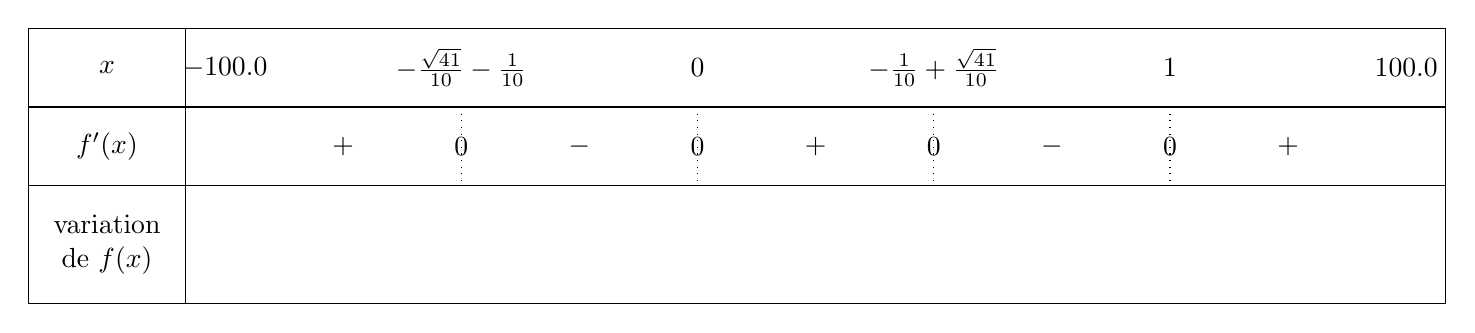
\begin{tikzpicture}
\tkzTabInit[espcl=3]{$x$ / 1 , $f'(x)$ / 1, variation de $f(x)$/1.5}
{$-100.0$,$- \frac{\sqrt{41}}{10} - \frac{1}{10}$,$0$,$- \frac{1}{10} + \frac{\sqrt{41}}{10}$,$1$,$100.0$}
\tkzTabLine{,+,z ,-,z ,+,z ,-,z ,+}
\tkzTabVar{-//+$-1.01 \cdot 10^{10}$,/+$\mathtt{\text{\$0.431\$}}$,/+$\mathtt{\text{\$0\$}}$,/+$\mathtt{\text{\$0.095\$}}$,/+$\mathtt{\text{\$0\$}}$,/+$9.9 \cdot 10^{9}$}
\end{tikzpicture}
\end{document}